\subsection{Composite}
\label{composite}

\textbf{Scopo}: Strutturale \\
\textbf{Raggio d'azione}: Oggetti

\paragraph{Definizione} Il pattern Composite permette di comporre oggetti in strutture ad albero per rappresentare gerarchie \textit{parte-tutto} e consentire ai client di trattare oggetti singoli e composizioni in modo uniforme.

\paragraph{Problema} Applicazioni quali editor grafici vettoriali o ambienti per la progettazione di circuiti consentono agli utenti di costruire diagrammi complessi a partire da semplici componenti. Componenti semplici possono essere raggruppati per costruire componenti più complessi che possono, a loro volta, essere utilizzati come parti di componenti ancor più complessi. Solitamente si introducono alcune classi per modellare gli oggetti semplici ed altre per rappresentare gli oggetti ottenuti per composizione.

\begin{figure}[H]
    \centering
    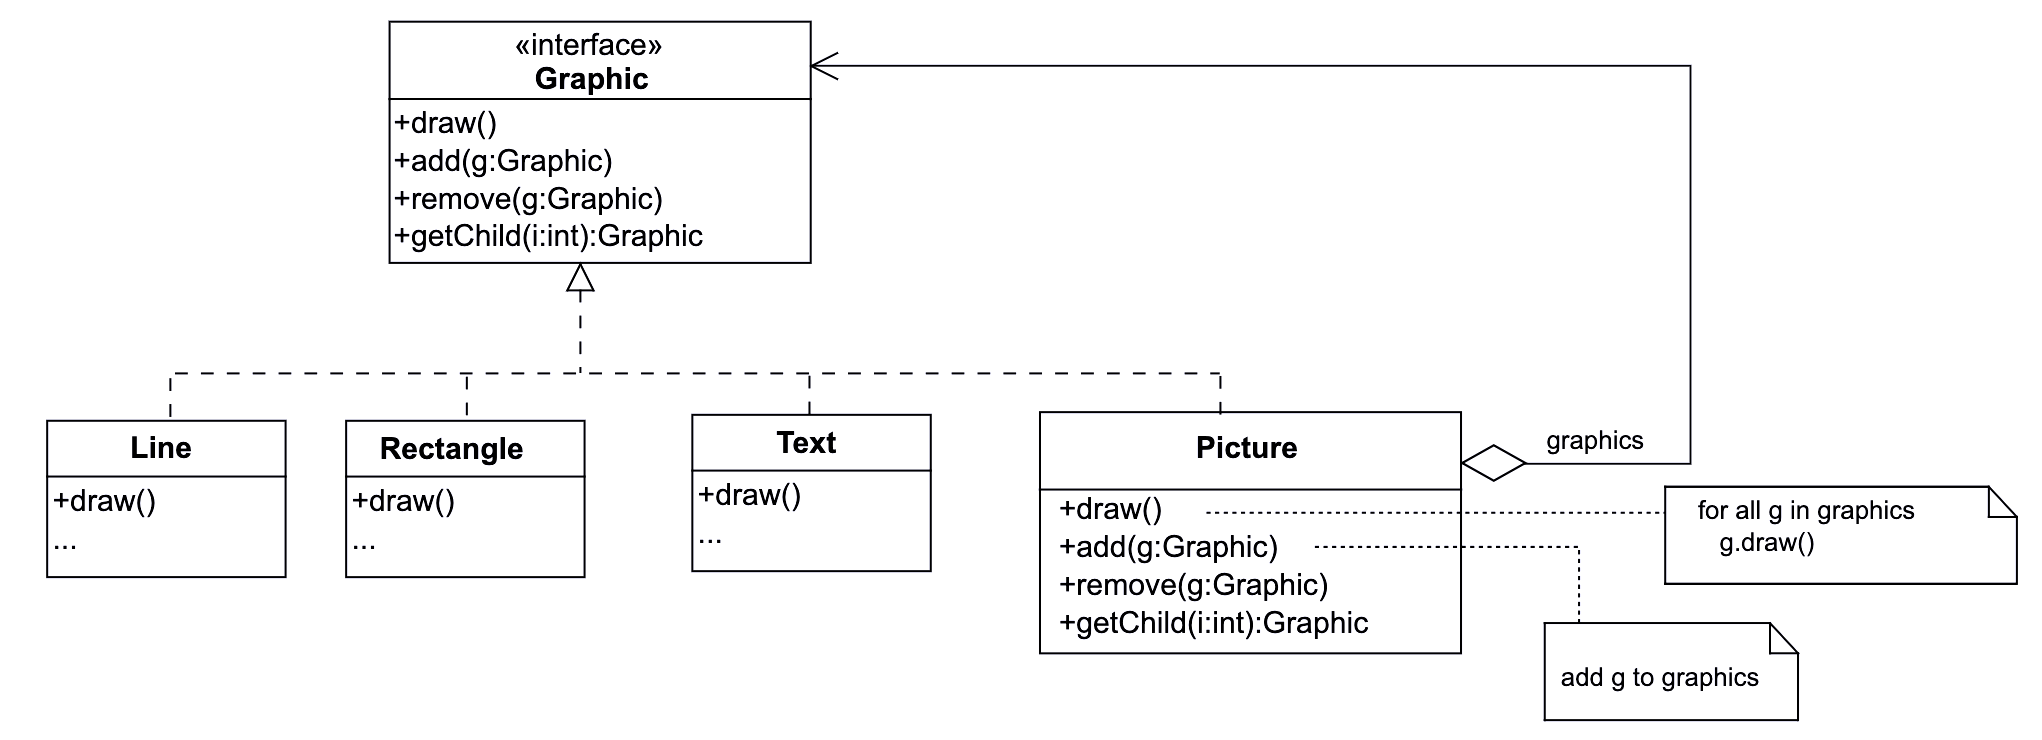
\includegraphics[width=0.8\linewidth]{assets/pattern/composite/composite-esempio.png}
\end{figure}

\paragraph{Soluzione} Il pattern Composite introduce un’interfaccia comune per gli oggetti semplici e per quelli compositi in modo che il codice cliente li possa trattare uniformemente. Nell’esempio, le classi Line, Rectangle e Text definiscono gli oggetti primitivi. Il metodo \textit{draw()} implementa l’operazione di disegno. Poichè gli oggetti primitivi non hanno figli, le operazioni per la gestione dei componenti non sono implementate. La classe Picture è un aggregato di oggetti Graphic ed implementa \textit{draw()} invocandolo a sua volta sugli oggetti da cui è composto.

\begin{figure}[H]
    \centering
    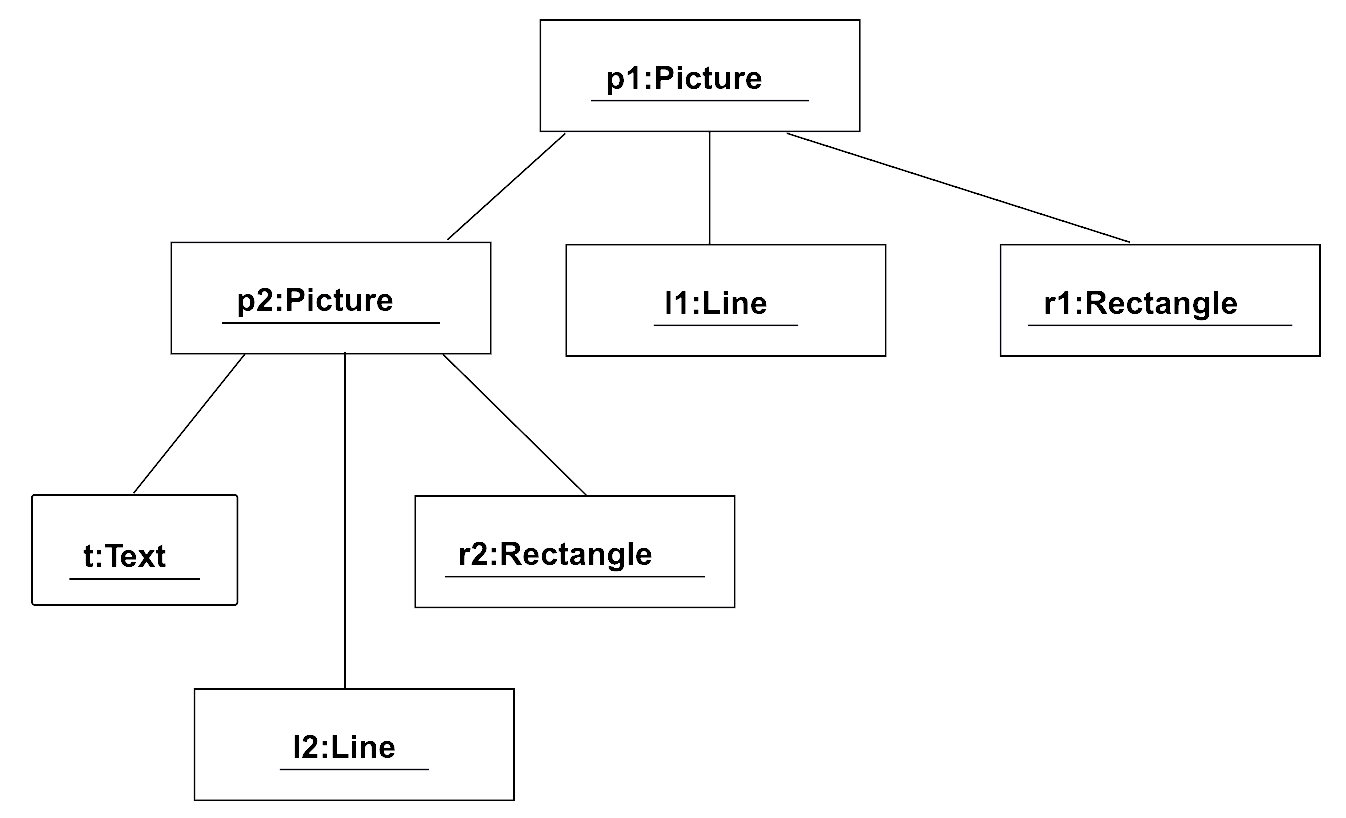
\includegraphics[width=0.5\linewidth]{assets/pattern/composite/composite-object.png}
    \caption{Tipica struttura di oggetti Graphic ricorsivamente composti}
\end{figure}

\newpage

\begin{figure}[H]
    \centering
    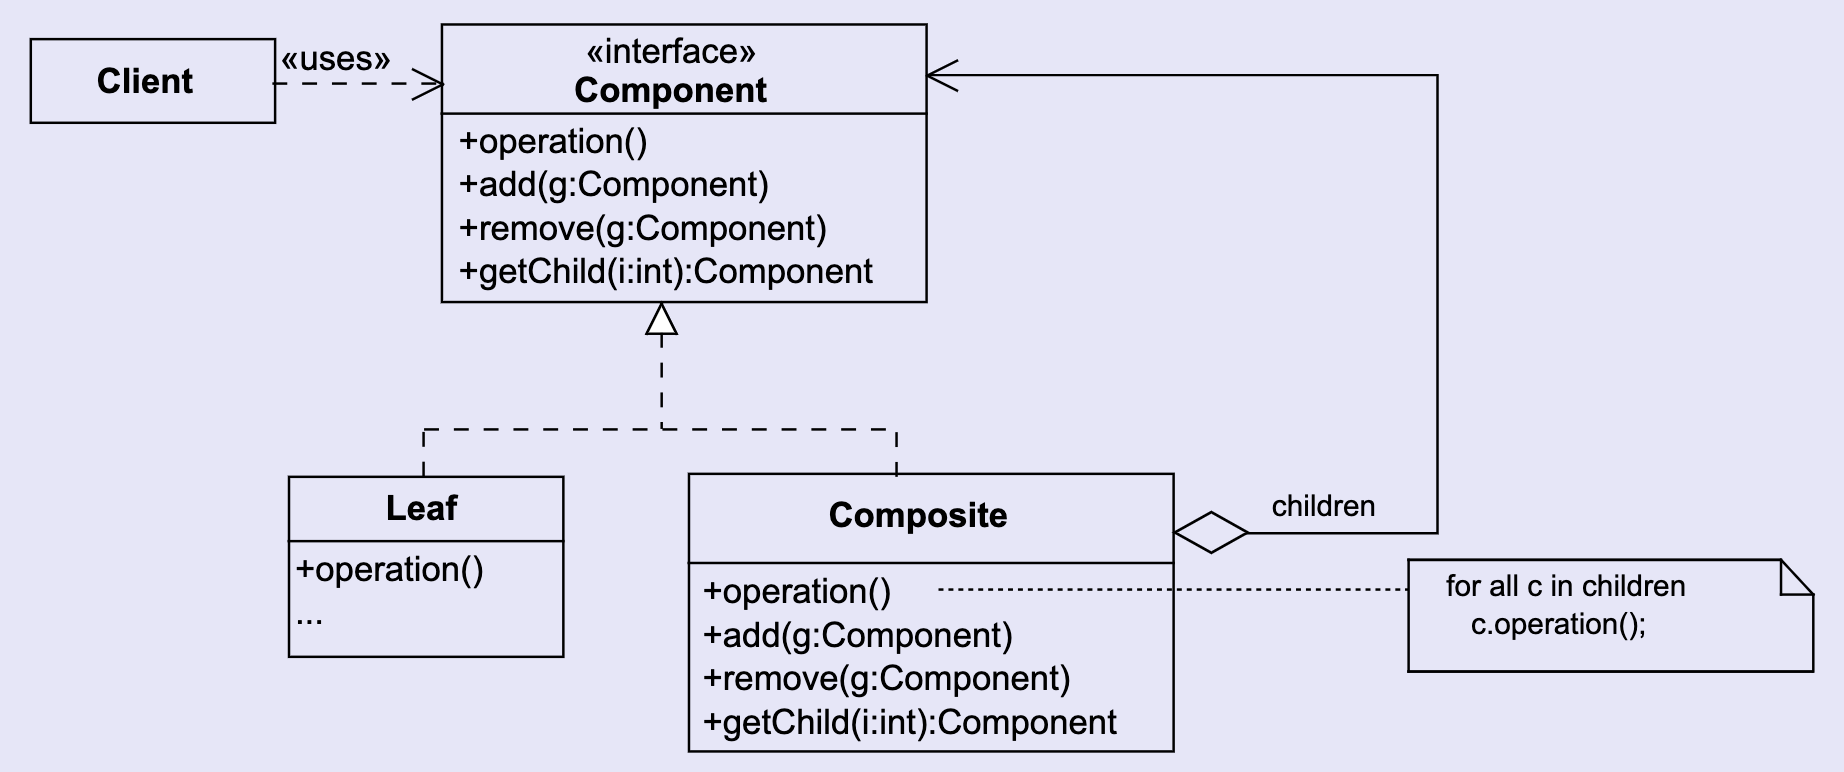
\includegraphics[width=1\linewidth]{assets/pattern/composite/composite-struttura.png}
\end{figure}

\paragraph{Struttura e Conseguenze} Il pattern composite è composto da:
\begin{itemize}
    \item \textbf{Component} (Graphic): dichiara l’interfaccia per gli oggetti componibili. Può essere una classe astratta che fornisce un’implementazione di default per i metodi di gestione dei componenti figli. Introduce (opzionale) un metodo per accedere al componente genitore. 
    \item \textbf{Leaf} (Rectangle,Line, etc.): rappresenta gli oggetti primitivi i quali non hanno figli. 
    \item \textbf{Composite} (Picture): definisce il comportamento dei componenti che hanno figli. Memorizza i componenti figli e implementa i relativi metodi introdotti dall’interfaccia Component.
\end{itemize}

\begin{figure}[H]
    \centering
    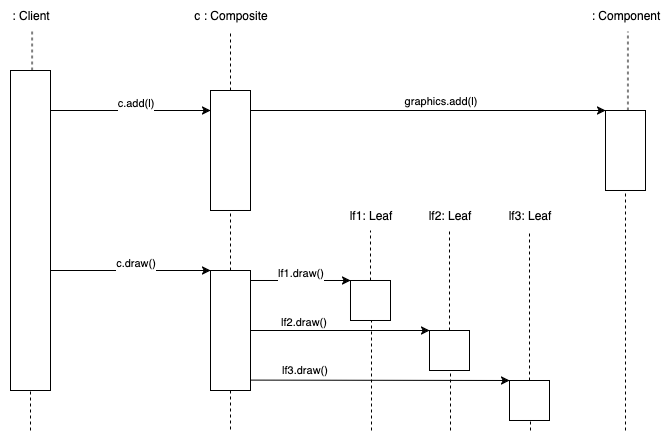
\includegraphics[width=1\linewidth]{assets/pattern/composite/composite-sequence.drawio.png}
\end{figure}

\newpage